% Szglab4
% ===========================================================================
%
\chapter{Analízis modell kidolgozása 2}

\thispagestyle{fancy}

\section{Objektum katalógus}

\subsection{Enemy}
Az \textbf{Enemy} osztály példányai egy-egy ellenséget tárolnak. Rendelkeznek típussal (fajjal), pillanatnyi pozícióval, hátralévő életerővel. Az idő haladtával próbálnak végighaladni egy véletlenszerűen választott lehetséges útvonalon.

\subsection{EnemyType}
Leírja egy ellenségtípus (jelen esetben a négy faj: ember, tünde, törp vagy hobbit) tulajdonságait, mint például az alapsebessége és a kezdeti életereje. Minden ellenségnek van egy referenciája egy példányára, amely meghatározza a viselkedését.

\subsection{Game}
Ez a játék logikáját magába foglaló osztály. Számon tartja a pályán lévő ellenfeleket, akadályokat és tornyokat, valamint végrehajtja a kiválasztott misszió által leírt forgatókönyvet, ami alapján az ellenségek érkeznek.

\subsection{Gem}
Egy épületekre rakható varázskő tulajdonságait tárolja. A \textbf{Game} osztály fog példányokat létrehozni belőle, különböző tulajdonságokkal. Ha egy épületre rá van rakva egy fajta varázskő, akkor az épület egy referenciát tárol a példányára.

\subsection{Map}
A \textbf{Map} a pályát képviseli, melyben NxM darab cella van. A pálya egy külső fájlból betölthető, ami új játék indulásakor fog megtörténni, miután kiválasztja a játékos a pályát. A pálya különböző tulajdonságai is lekérdezhetőek, amelyek majd a kirajzoláshoz kellenek.

\subsection{Mission}
Egy \textbf{Mission} objektumban lesz eltárolva, hogy milyen ellenségek, mikor és honnan jönnek be a pályára. Ez a három adat majd egy segéd osztályban lesz összefogva, és egy tárolóban lesz tárolva. A játék főciklusa le tudja majd kérdezni a következő ellenséget, melyet az objektum visszaad, ha már elég idő eltelt az előző egység óta (ha nem akkor nem ad vissza egységet).

\subsection{Obstacle}
Egy akadályt valósít meg. Ha egy ellenség belelép egy olyan mezőbe, amin van egy \textbf{Obstacle}, akkor azt egy bizonyos mértékben lelassítja, az ellenség fajától függően.

\subsection{Projectile}
Ez az osztály egy lövedék leírása. Amikor egy torony lő, akkor példányosítja ezt az osztályt a cél ellenség átadásával, így egy lövedék mindig a torony által meghatározott ellenség után megy, amit ha megfelelően megközelít (eltalálja az ellenséget), akkor levesz az életerejéből és megsemmisíti magát.

\subsection{Tile}
A \textbf{Tile} objektumból egy NxM-es tömböt fog tárolni a \textbf{Map} objektum. Ezek a pálya egyes celláit fogják képviselni. Egy cellán lehet maximum egy darab épület, amely vagy egy torony, vagy egy akadály, attól függően, hogy van-e a cellán út, vagy nincsen. A cellán levő épület referenciája lekérhető, vagy ha még nincsen rajta, és a cellára kattintás történik, akkor épül egy megfelelő épület.\\
Ha egy cellán van út, akkor lekérdezhető, hogy az a cella milyen távol van a céltól (az utat követve, cellákban mérve). Továbbá az is tárolva van, és lekérdezhető, hogy az út merre folytatódik (és az ellenségeknek merre kell majd menniük). Ha elágazás van, akkor véletlenszerűen választ irányt és arra küldi az ellenséget (ez minden egyes ellenségre véletlenszerű).

\subsection{Tower}
Egy tornyot valósít meg. Ha egy ellenség a hatókörébe ér, akkor elindít egy \textbf{Projectile}-t az irányába, a tüzelési gyakoriságának megfelelő időközönként. Ha több ellenfél van a hatókörében, akkor arra lő, aki a legközelebb van a célhoz.


\section{Statikus struktúra diagramok}

\begin{figure}[H]
\begin{center}
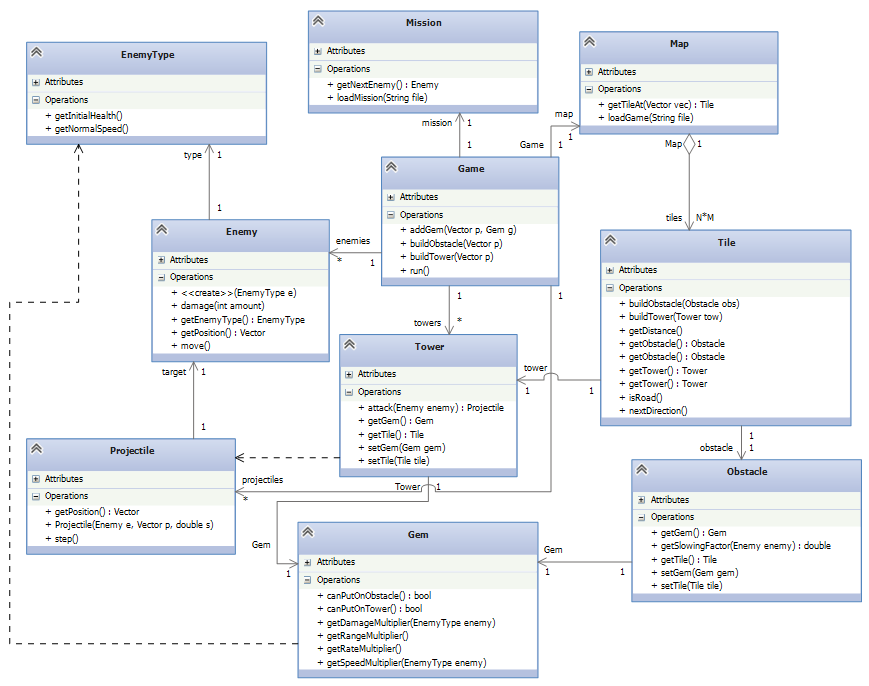
\includegraphics[width=17cm]{images/class.png}
\caption{Osztálydiagram}
\label{fig:class_diag}
\end{center}
\end{figure}


\section{Osztályok leírása}


\subsection{Enemy}
\begin{itemize}
\item Felelősség\\
Az ellenségek pozíciójának, sebességének és életerejének nyilvántartása.
\item Attribútumok
	\begin{itemize}
		\item \textbf{EnemyType} type: Az egység típusa.
		\item double health: Az ellenség fennmaradó életereje.
		\item \textbf{Vector} position: Pillanatnyi pozíció a pályán.
	\end{itemize}
\item Metódusok
	\begin{itemize}
		\item boolean move(double dt): Az egységet annyival mozgatja az útján tovább, amennyit dt idő alatt halad. Ha az ellenség életereje 0 vagy kisebb, akkor true-val tér visza, egyébként false-al.
		\item \textbf{Vector} getPosition(): A position attribútum értékével tér vissza.
		\item boolean damage(double amount): Csökkenti az ellenség életerejét amount-al, igazzal tér vissza ha az ellenség meghalt.
		\item \textbf{EnemyType} getEnemyType(): Visszaadja az ellenség típusát.
	\end{itemize}
\end{itemize}


\subsection{EnemyType}
\begin{itemize}
\item Felelősség\\
Leírja egy bizonyos típusú (fajú) ellenség alapvető tulajdonságait. Egy-egy példányára hivatkozik az összes ellenség, amelyeknek ezáltal meghatározza a viselkedését.
\item Attribútumok
	\begin{itemize}
		\item int cost: Az ilyen fajtájú ellenségek ára varázserőben.
		\item double initialHealth: Az ilyen fajtájú ellenségek kezdeti életereje.
		\item double normalSpeed: Az ilyen fajtájú ellenségek akadályoztatás nélküli haladási sebessége.
	\end{itemize}
\item Metódusok
	\begin{itemize}
		\item double getInitialHealth(): Visszaadja az initialHealth attribútum értékét.
		\item double getNormalSpeed(): Visszaadja a normalSpeed attribútum értékét.
	\end{itemize}
\end{itemize}




\subsection{Game}
\begin{itemize}
\item Felelősség\\
A többi osztály nyilván tartása és összekötése, a játékbeli események vezérlése. A felhasználói felülettől érkező parancsok végrehajtása, és a játék állapotának rendelkezésre bocsájtása a kijelzéshez.
\item Attribútumok
	\begin{itemize}
		\item \textbf{ArrayList}<\textbf{Projectile}> projectiles: Eltárolja a jelenleg játékban lévő lövedékeket.
		\item \textbf{Map} map: Referencia a kiválasztott pályára, amin a játék folyik.
		\item \textbf{Mission} mission: Referencia a kiválasztott misszióra, amely alapján zajlik a játék.
		\item \textbf{ArrayList}<\textbf{Building}> buildings: Eltárolja a játékos megépített tornyait.
		\item \textbf{ArrayList}<\textbf{Gem}> gems: Az összes lehetséges, toronyra illetve akadályra rakható varázskő nyilvántartása.
		\item \textbf{ArrayList}<\textbf{EnemyType}> types: Ez a lehetséges ellenségtípusok listája.
		\item \textbf{ArrayList}<\textbf{Enemy}> enemies: Az összes éppen látható ellenség található meg benne.
		\item int magic: A játékos jelenlegi varázsereje.
	\end{itemize}
\item Metódusok
	\begin{itemize}
		\item void run(): Ez a metódus futtatja a főciklust, amelyben maga a játék működik.
		\item void buildTower(\textbf{Vector} position): Épít egy tornyot a paraméterül kapott helyen évő mezőre.
		\item void buildObstacle(\textbf{Vector} position): Épít egy akadályt a paraméterül kapott helyen lévő mezőre.
		\item void addGem(\textbf{Vector} position, \textbf{Gem} gem): A paraméterként kapott helyen lévő toronyra vagy akadályra rárakja a paraméterként kapott varázskövet.
	\end{itemize}
\end{itemize}




\subsection{Gem}
\begin{itemize}
\item Felelősség\\
Egy fajta varázskő tulajdonságainak tárolása.
\item Attribútumok
	\begin{itemize}
		\item int cost: A varázskő ára varázserőben.
		\item double rangeMultiplier: Megadja, hogy a varázskővel ellátott toronynak hányszorosára nő a hatótávolsága.
		\item double rateMultiplier: Megadja, hogy a varázskővel ellátott toronynak hányszorosára nő a tüzelési sebessége.
		\item \textbf{HashMap}<\textbf{EnemyType}, \textbf{Double}> damageMultiplier: Megadja, hogy a varázskővel ellátott toronynak hányszorosára nő a sebzése egy adott típusú ellenséggel szemben.
		\item \textbf{HashMap}<\textbf{EnemyType}, \textbf{Double}> speedMultiplier: Megadja, hogy a varázskővel elátott akadályon áthaladó adott típusú ellenség sebessége hányadára csökken.
	\end{itemize}
\item Metódusok
	\begin{itemize}
		\item \textbf{Gem}(double rangeMultiplier, double rateMultiplier, \textbf{HashMap}<\textbf{EnemyType}, Double> damageMultiplier, \textbf{HashMap}<\textbf{EnemyType}, \textbf{Double}> speedMultiplier): Létrehoz egy \textbf{Gem} objektumot a paraméterként kapott tulajdonságokkal.
		\item double getRangeMultiplier(): Visszaadja a varázskő hatótávolság szorzóját.
		\item double getRateMultiplier(): Visszaadja a varázskő tüzelési sebesség szorzójáz.
		\item double getDamageMultiplier(\textbf{EnemyType} enemyType): Visszaadja varázskő sebzés szorzóját egy adott típusú ellenséghez.
		\item double getSpeedMultiplier(\textbf{EnemyType} enemyType): Visszaadja varázskő sebesség szorzóját egy adott típusú ellenséghez.
		\item boolean canPutOnTower(): Ha a varázskő használható tornyokra, igazat ad vissza, különben hamisat.
		\item boolean canPutOnObstacle() Ha a varázskő használható akadályokra, igazat ad vissza, különben hamisat.
	\end{itemize}
\end{itemize}


\subsection{Map}
\begin{itemize}
\item Felelősség\\
Tartlamaz az összes cellára referenciát, felelős a kapott fájlból beolvasni a pályát, és felépíteni azt.
\item Attribútumok
	\begin{itemize}
		\item \textbf{Tile}[][] tiles: A pályán található cellák tömbje, a pálya kirajzolásához használható.
	\end{itemize}
\item Metódusok
	\begin{itemize}
		\item \textbf{Tile} getTileAt(\textbf{Vector} position): Visszaadja a position helyen talalható cellát.
		\item loadGame(\textbf{String} file): Betölti a kapott elérési útvonalon a fájlt, és felépíti az alapján a pályát.
	\end{itemize}
\end{itemize}


\subsection{Mission}
\begin{itemize}
\item Felelősség\\
Felelőssége, felépíteni a listát, amely a beérkező ellenségeket és időzítésüket tartalmazza. Majd a megfelelő időközönként ki kell adja ezeket az egységeket a \textbf{Game} osztálynak.
\item Attribútumok
	\begin{itemize}
		\item \textbf{List}<\textbf{Spawn}> spawnList: A Spawn segédosztályban tárolt ellenség-idő-belépési pont, adatokat tárolja.
		\item double lastSpawn: Tárolja az előző spawn idejét.
	\end{itemize}
\item Metódusok
	\begin{itemize}
		\item \textbf{Enemy} getNextEnemy(double time): A spawnList listaból a következő elemet megvizsgaálja, és ha spawnolni kell a következő ellenséget, akkor visszaadja azt.
		\item loadMission(\textbf{String} file): Betölti a kapott elérési útvonalon a fájlt, és felépíti az alapján a listát (spawnList).
	\end{itemize}
\end{itemize}


\subsection{Obstacle}
\begin{itemize}
\item Felelősség\\
Felelős \textbf{Projectile}-ok létrehozásához, azok megfelelő felparaméterezésével. Továbbá felelős azért, hogy \textbf{Projectile}-okat csak a megadott időközönként lőjjön ki.
\item Attribútumok
		\item \underline{int cost}: Az akadály ára varázserőben.
		\item \textbf{Gem} gem: Eltárol egy referenciát egy \textbf{Gem} típusú objektumra, ami meghatározza, hogy az adott épület milyen echant alatt áll.
		\item \textbf{Map}<\textbf{EnemyType}, double> speedMultiplier: Megadja mekkora az adott típusú ellenfélre kifejtett hatása az akadálynak.
		\item \textbf{Tile} tile: Egy referencia arra a mezőre, ahol az épület található.
\item Metódusok
	\begin{itemize}
		\item double getSlowingFactor(\textbf{Enemy} enemy): Visszatér azzal az értékkel, amivel az adott ellenfelet lassítja.
		\item \textbf{Gem} getGem(): Visszaadja az épületen található varázskövet.
		\item void setGem(\textbf{Gem} gem): Beállítja az epületen lévő varázskövet. Ha már volt az épületen varázskő, akkor az előző megszűnik.
		\item void setTile(\textbf{Tile} tile): Beállítja, hogy az akadály melyik \textbf{Tile}-on van.
		\item \textbf{Tile} getTile(): Visszaadja, hogy az akadály melyik \textbf{Tile}-on van.
	\end{itemize}
\end{itemize}


\subsection{Projectile}
\begin{itemize}
\item Felelősség\\
Követni a cél ellenséget, majd sebezni ha eléri.
\item Attribútumok
	\begin{itemize}
		\item double damage: A lövedék sebzése, ennyivel csökkenti a cél ellenség életerejét amikor eltalálja.
		\item \textbf{Vector} position: A lövedék pozíciója.
		\item double speed: A lövedék sebessége.
		\item \textbf{Enemy} enemy: A lövedék cél \textbf{Enemy}-je.
	\end{itemize}
\item Metódusok
	\begin{itemize}
		\item Projectile(\textbf{Enemy} enemy, \textbf{Vector} position, double speed): Konstruktor, átveszi a cél \textbf{Enemy}-t, a kezdő pozíciót és sebességet.
		\item boolean move(double dt): dt * speed-el mozgatja a lövedéket az ellenség irányába. Ha eltalálta az ellenséget vagy az ellenség már meghalt, akkor true-t ad vissza, különben false-t.
		\item \textbf{Vector} getPosition(): Visszaadja a lövedék pozícióját.
	\end{itemize}
\end{itemize}


\subsection{Tile}
\begin{itemize}
\item Felelősség\\
Egy cellán lehet maximum egy darab épület, amely vagy egy torony, vagy egy akadály, attól függően, hogy van-e a cellán út, vagy nincsen. A cellán levő épület referenciája lekérhető, vagy ha még nincsen rajta, és a cellára kattintás történik, akkor épül egy megfelelő épület. Felelős még az egyes ellenségek következő irányának a meghatározására, és vissza kell tudnia adni, hogy van-e rajta út, valamint ha van akkor milyen távol van a céltól.
\item Attribútumok
	\begin{itemize}
		\item \textbf{Building} building: A cellában levő epület.
		\item int distance: Hányadik cella az utat követve a céltól.
		\item boolean road: Van-e út a cellában.
		\item double up: Annak a valószinűsége, hogy a cellából felfelé fog menni az ellenség.
		\item double down: Annak a valószinűsége, hogy a cellából lefelé fog menni az ellenség.
		\item double left: Annak a valószinűsége, hogy a cellából balra fog menni az ellenség.
		\item double right: Annak a valószinűsége, hogy a cellából jobbra fog menni az ellenség.
	\end{itemize}
\item Metódusok
	\begin{itemize}
		\item void buildTower(): A cellán egy tornyot épít.
		\item void buildObstacle(): A cellán egy akadályt épít.
		\item \textbf{Tower} getTower(): Visszaadja a cellán lévő tornyot.
		\item \textbf{Obstacle} getObstacle(): Visszaadja a cellán lévő akadályt.
		\item int getDistance(): Visszaadja a distance értékét.
		\item boolean isRoad(): Visszaadja a road értékét.
		\item \textbf{Direction} nextDirection(): Visszad egy irány enum-ot, amely megadja az ellenség irányát.
	\end{itemize}
\end{itemize}


\subsection{Tower}
\begin{itemize}
\item Felelősség\\
Felelős \textbf{Projectile}-ok létrehozásához, azok megfelelő felparaméterezésével. Továbbá felelős azért, hogy \textbf{Projectile}-okat csak a megadott időközönként lőjjön ki.
\item Attribútumok
	\begin{itemize}
		\item \underline{int cost}: A torony ára varázserőben.
		\item \textbf{Gem} gem: Eltárol egy referenciát egy \textbf{Gem} típusú objektumra, ami meghatározza, hogy az adott épület milyen echant alatt áll.
		\item \textbf{HashMap}<\textbf{EnemyType}, double> damage: Megadja mekkora az adott típusú ellenfélre kifejtett hatása a toronynak.
		\item \textbf{Tile} tile: Egy referencia arra a mezőre, ahol az épület található.
	\end{itemize}
\item Metódusok
	\begin{itemize}
		\item \textbf{Projectile} attack(\textbf{Enemy} enemy): Kilő egy \textbf{Projectile}-t a paraméterként megkapott ellenségre, majd a visszatérési értékében visszaadja azt. A \textbf{Projectile}-t felparaméterezi az ellenséghez megfelelő sebzési adatokkal.
		\item \textbf{Gem} getGem(): Visszaadja az épületen található varázskövet.
		\item void setGem(\textbf{Gem} gem): Beállítja az epületen lévő varázskövet. Ha már volt az épületen varázskő, akkor az előző megszűnik.
		\item void setTile(\textbf{Tile} tile): Beállítja, hogy a torony melyik \textbf{Tile}-on van.
		\item \textbf{Tile} getTile(): Visszaadja, hogy a torony melyik \textbf{Tile}-on van.
	\end{itemize}
\end{itemize}


\section{Szekvencia diagramok}

\begin{figure}[H]
\begin{center}
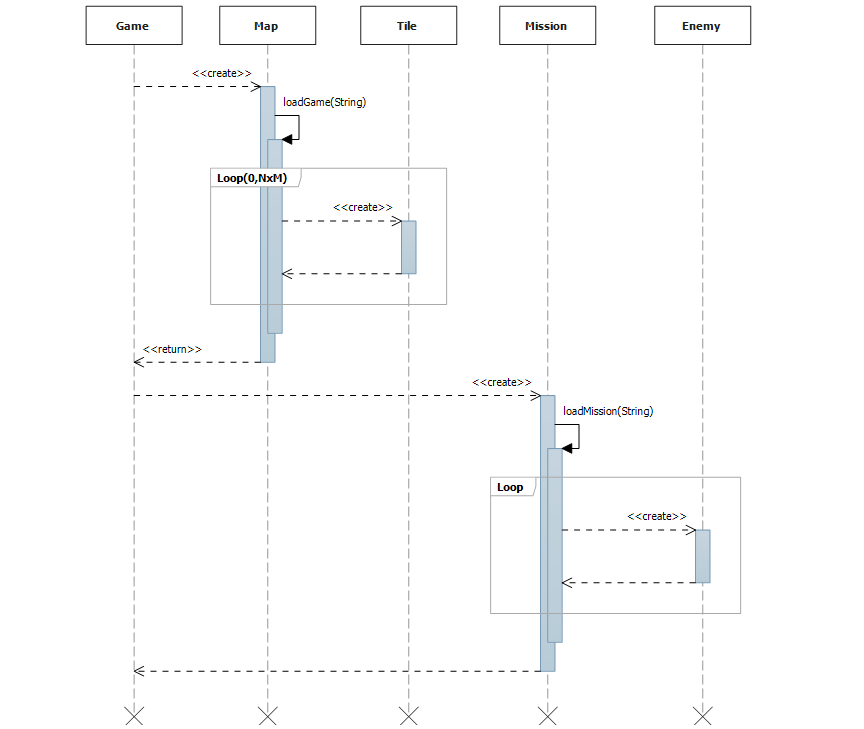
\includegraphics[width=15cm]{images/starting_game.png}
\caption{Játék indítása}
\label{fig:starting_game}
\end{center}
\end{figure}

\begin{figure}[H]
\begin{center}
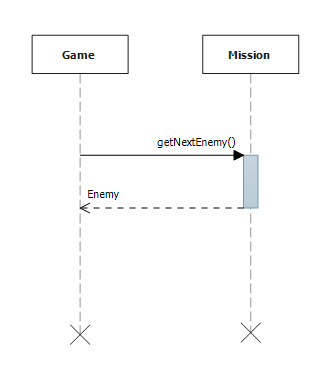
\includegraphics[width=10cm]{images/scheduling_enemies.png}
\caption{Ellenségek ütemezése}
\label{fig:scheduling_enemies}
\end{center}
\end{figure}

\begin{figure}[H]
\begin{center}
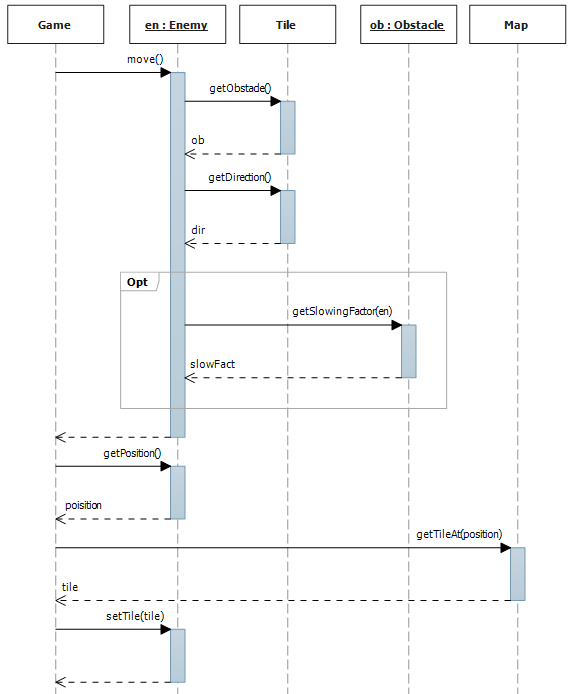
\includegraphics[width=13cm]{images/moving_enemy.png}
\caption{Ellenség mozgatása}
\label{fig:moving_enemy}
\end{center}
\end{figure}

\begin{figure}[H]
\begin{center}
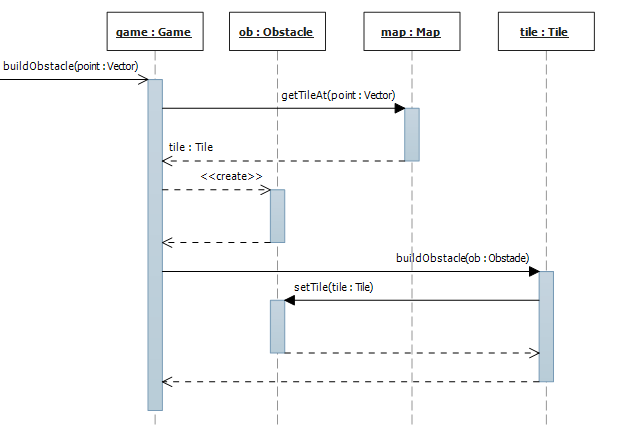
\includegraphics[width=15cm]{images/building_obstacle.png}
\caption{Akadály építése}
\label{fig:building_obstacle}
\end{center}
\end{figure}

\begin{figure}[H]
\begin{center}
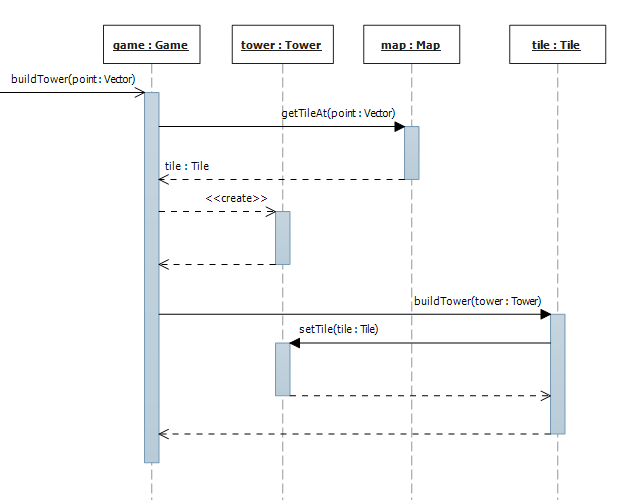
\includegraphics[width=15cm]{images/building_tower.png}
\caption{Torony építése}
\label{fig:building_tower}
\end{center}
\end{figure}

\begin{figure}[H]
\begin{center}
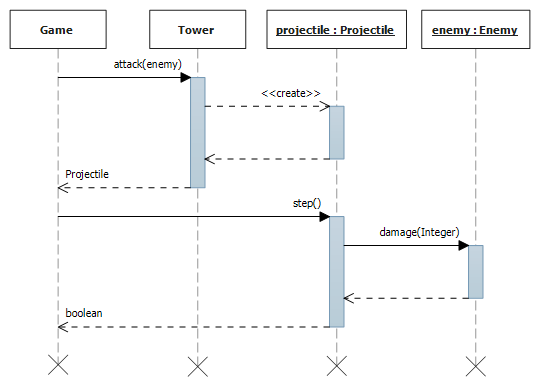
\includegraphics[width=15cm]{images/tower_firing.png}
\caption{Torony tüzelése}
\label{fig:tower_firing}
\end{center}
\end{figure}

\begin{figure}[H]
\begin{center}
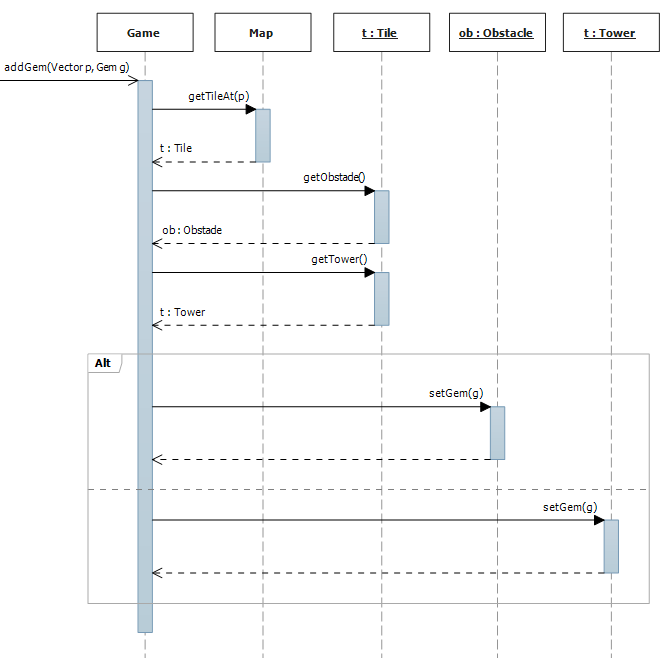
\includegraphics[width=15cm]{images/adding_gem.png}
\caption{Varázskő feltétele}
\label{fig:adding_gem}
\end{center}
\end{figure}

\begin{figure}[H]
\begin{center}
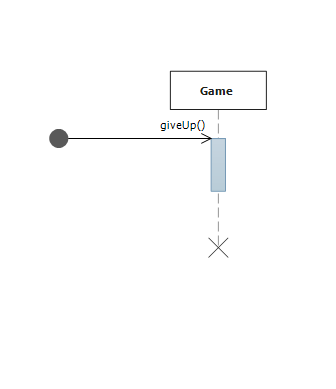
\includegraphics[width=10cm]{images/giving_up.png}
\caption{Feladás}
\label{fig:giving_up}
\end{center}
\end{figure}


\pagebreak
\section{State-chartok}

\begin{figure}[H]
\begin{center}
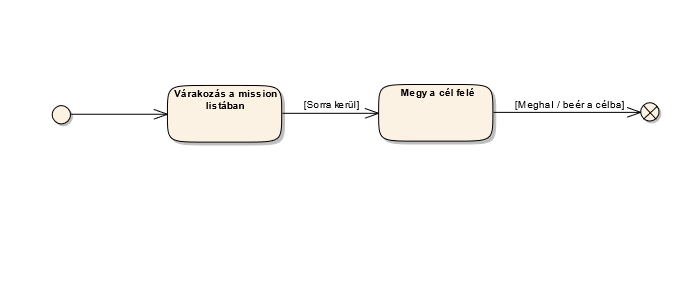
\includegraphics[width=15cm]{images/enemy_state.png}
\caption{Egy ellenség állapotdiagramja}
\label{fig:enemy_state}
\end{center}
\end{figure}

\begin{figure}[H]
\begin{center}
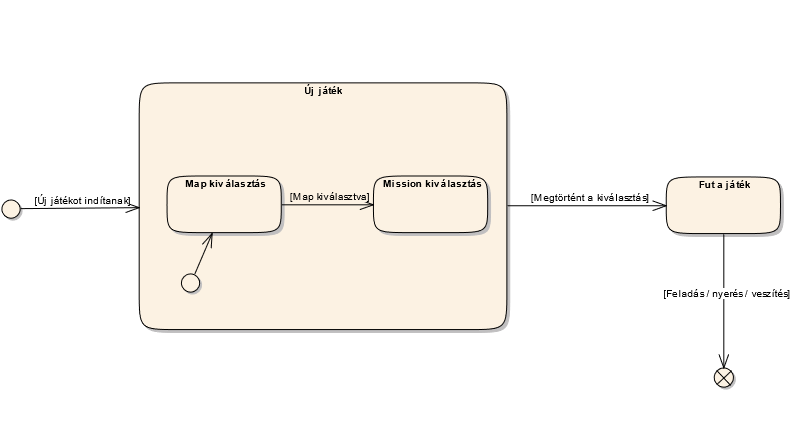
\includegraphics[width=15cm]{images/game_state.png}
\caption{A játék állapotdiagramja}
\label{fig:game_state}
\end{center}
\end{figure}

\begin{figure}[H]
\begin{center}
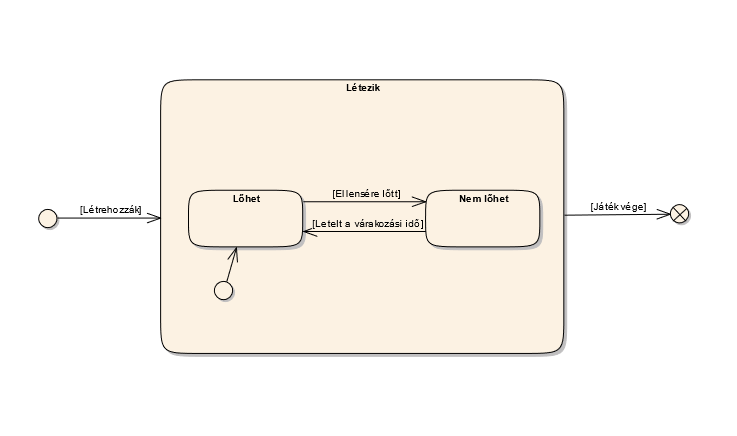
\includegraphics[width=15cm]{images/tower_state.png}
\caption{Egy torony állapotdiagramja}
\label{fig:tower_state}
\end{center}
\end{figure}

